這一節的UB,是由開發者指定的。要做到這一點,首先需要從不同的角度來考慮UB。 

到目前為止,看到的所有UB的例子都可以分為兩種。第一類是像\texttt{++k +k}表達式這樣的代碼,這些都是錯誤,因為其根本沒有定義行為。第二種是像\texttt{k + 1}這樣的代碼,其中\texttt{k}是有符號整數。這中代碼到處都是,而且大多數時候,都工作得很好。除了變量為特定的某些值外,它的行為有良好的定義。

換句話說,代碼具有隱式的先決條件,只要滿足了這些先決條件,程序就會表現良好。注意,在更大程序的上下文中,這些先決條件可能是隱式的。程序可能驗證輸入或中間結果,並防範可能導致UB的值。無論採用哪種方式,開發者都與用戶有了一種約定:如果輸入符合某些限制,則保證結果是正確的,並且程序可以以一種定義良好的方式運行。

如果違反了限制會發生什麼?有以下兩種可能:

\begin{itemize}
\item 
首先,程序可能檢測到輸入不符合約定,並處理錯誤。這種行為仍然得到了很好的定義,並且是規範的一部分。

\item 
其次,程序可能無法檢測到約定被違反,並像往常一樣繼續進行。由於約定對於保證正確的結果至關重要,所以現在在未知的領域運行,而且沒有辦法預測將會發生什麼。
\end{itemize}

這就是UB的描述。

既然已經理解了UB僅是在指定的約定之外運行的程序的行為,那麼可以考慮一下如何將其在應用中使用。

大多數足夠複雜的程序在其輸入上都有先決條件,即與用戶進行約定。有人可能會說,應該總是檢查這些先決條件,並報告錯誤。然而,這可能是一個非常昂貴的需求。再來看一個例子。

要編寫一個程序來掃描畫在一張紙上(或蝕刻在印刷電路板上)的圖像,並將其轉換為圖形數據。程序的輸入可能是這樣的:

%\hspace*{\fill} \\ %插入空行
\begin{center}
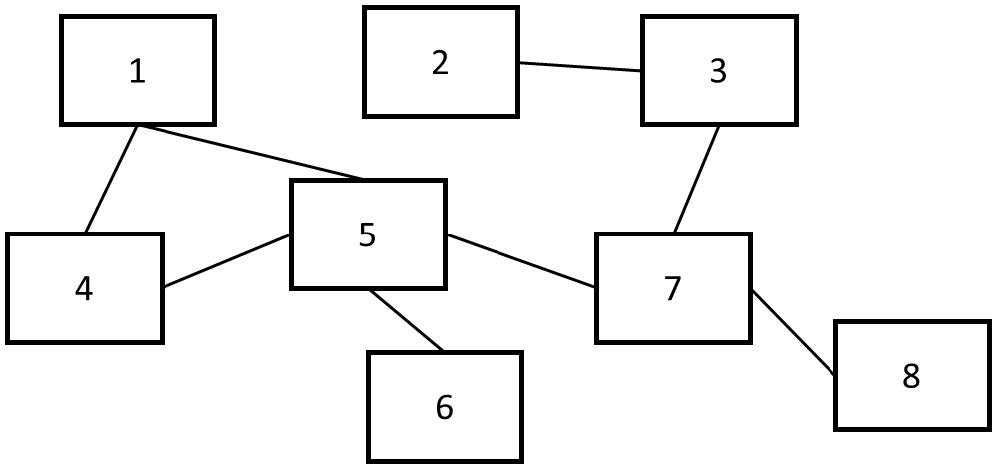
\includegraphics[width=0.9\textwidth]{content/3/chapter11/images/8.jpg}\\
圖11.8 - 圖形繪製是圖形程序的輸入
\end{center}

程序獲取圖像,識別矩形,從每個矩形創建圖形節點,識別直線,為每條直線找出它連接的兩個矩形,並在圖形中創建相應的邊。

假設有一個圖像採集和分析庫,提供一組形狀(矩形和直線)及其所有座標,所以現在要做的就是找出哪些直線連接哪些矩形。有了所有的座標,所以從現在開始,問題就是純幾何的。表示這個圖最簡單的方法之一是用邊表表示。可以使用容器(比如,\texttt{vector})作為表,如果給每個節點分配唯一的數字ID,一條邊就是一對數字。可以使用任意數量的幾何算法來檢測直線和矩形之間的交點,並逐邊構造這個表(以及圖本身)。

聽起來很簡單,有一個數據的自然表示,相當簡單,並容易處理。不幸的是,這裡還與用戶有一個隱式約定:要求每條線恰好與兩個矩形相交(同樣,矩形也不互相相交,避免混亂)。 

%\hspace*{\fill} \\ %插入空行
\begin{center}
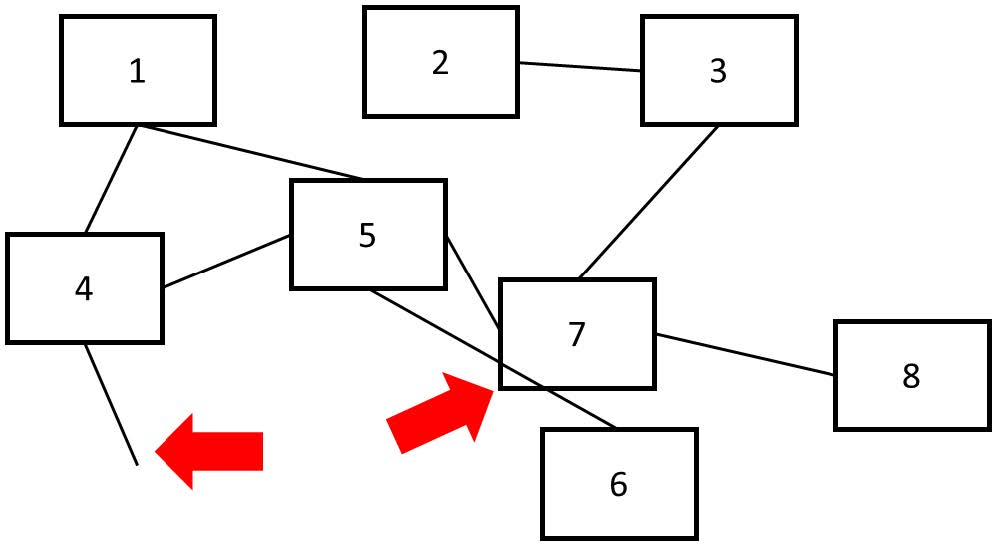
\includegraphics[width=0.9\textwidth]{content/3/chapter11/images/9.jpg}\\
圖11.9 - 圖形識別程序的無效輸入
\end{center}

圖11.9中,看到了一個違反約定的輸入:其中一條線連接了三個矩形,而另一條線只連接了一個矩形。如前所述,有兩個選擇:可以檢測並報告輸入錯誤,或者可以忽略。第一個選項使程序健壯,但會有性能損失:原始程序可能會在找到第二個這樣的矩形後,停止尋找連接到給定邊的矩形,並從那時起忽略這條邊。這種優化的收益是相當可觀的:對於類似於圖11.8(但要大得多)的圖,可以將運行時間減少一半。如果輸入最終是正確的,那麼強制輸入驗證會浪費大量時間,並且會讓有其他方法確保輸入有效的用戶感到沮喪。不驗證輸入將導致UB:如果有一條線連接三個矩形,算法將在找到前兩個矩形後停止,無論它處理它們的順序是什麼(這個順序可能是依賴於數據的,所以對於這種情況,可以說的是在涉及的兩個節點之間將創建了一條邊)。

如果性能差異不明顯(或者總體運行時間很短,所以翻倍也不重要),那麼最好的解決方案就很明顯——驗證輸入。在這種情況和許多其他情況下,驗證的成本很容易與找到解決方案一樣高。在這種情況下應該怎麼做呢?

首先,必須清楚強加給用戶的約定。應該清楚地指定,並記錄什麼是有效的輸入。在此之後,性能敏感型項目的最佳實踐是提供最佳性能。更廣泛的約定(施加更少限制的約頂)總是比狹義的約定好,所以如果有一些無效輸入,可以很容易地檢測,並以最小的開銷處理它們,那麼就應該這樣做。除此之外,能做的就是記錄程序行為未定義時的條件,就像C++標準一樣。 

還可以做一些努力,可以為用戶提供一個輸入驗證工具,既可以作為程序中的一個可選步驟,也可以作為單獨的軟件。運行它需要時間,但是如果用戶從主程序中得到了奇怪的結果,可以使用工具檢查,以確保輸入是有效的。這比在行為未定義時簡單地描述要好得多(然而,在有些情況下,這樣的驗證開銷太大,反而不實用)。

如果C++編譯器開發人員會做同樣的工作,並提供一個可選的工具來檢測代碼中的UB,豈不妙哉?事實證明,開發人員也是這麼想的:今天許多編譯器都有一個選項來啟用UB殺滅器(通常稱為UBSan)。讓我們從一些可以導致UB的代碼開始瞭解其工作原理:

\begin{lstlisting}[style=styleCXX]
int g(int k) {
	return k + 10;
}

\end{lstlisting}

編寫一個程序,用足夠大的參數(大於\texttt{INT\_MAX-10})調用這個函數,並在啟用UBSan的情況下編譯它。對於Clang或GCC,該選項是\texttt{-fsanitize=undefined}。這裡有一個例子:

\begin{tcblisting}{commandshell={}}
clang++ --std=c++17 –O3 –fsanitize=undefined ub.C
\end{tcblisting}

運行該程序,就會看到如下內容:

\begin{tcblisting}{commandshell={}}
ub.C:10:20: runtime error: signed integer overflow: 
        2147483645 + 10 cannot be represented in type 'int'
\end{tcblisting}

就像在我們的圖形示例中一樣,UB檢測需要時間,並且會使程序變慢,所以這應該在測試和調試時去做的事情。讓殺滅器運行常規迴歸測試的一部分,並認真對待報告的錯誤:雖然今天生成了正確的結果,但並不意味著明天下一個編譯器不會生成一些非常不同的代碼,並更改結果。

我們已經瞭解了UB,為什麼它有時是一種必要的惡,以及如何利用它來提高性能。結束這一章之前,讓我們回顧一下我們瞭解過的東西。

























